\documentclass[11pt,a4paper]{article}
\usepackage[margin=1.8cm]{geometry}
\usepackage{amsmath,amssymb,booktabs,graphicx,array,longtable}
\usepackage[hidelinks]{hyperref}
\usepackage{microtype}
\hypersetup{pdftitle={Fiducial ttW production-decay scale comparison, 30 October 2026},
pdfauthor={ttW production-decay study}}
\setlength{\parindent}{0pt}
\setlength{\parskip}{0.45em}
\graphicspath{{figures/}}
\newcommand{\pt}{p_{\mathrm T}}
\newcommand{\code}[1]{\texttt{\detokenize{#1}}}
\title{Production--decay scale correlations and width conventions\\
in fiducial trileptonic $t\bar tW^+$ production\\
\large Updated comparison from forty completed integrations}
\author{ttW production--decay study}
\date{30 October 2026}
\begin{document}
\maketitle
\begin{abstract}
We combine ten repeated integrations for each of four predictions:
additive ($S$) or multiplicative ($\Pi$) NLO QCD production and top decays,
with scale-dependent or fixed total widths. The samples use the updated
common lepton selection, applied during generation, and retain 581
histograms and all 81 production/decay scale combinations. The selected
total rates agree at the 0.13\% level, while $\Pi$ increases the exclusive
zero- and one-bottom-jet rates by approximately 16.8\% and 7.8\%, and
decreases the two-tag rate by 4.0\%. For the two-tag multiplicative
prediction with fixed widths, the scale envelope is
${}^{+7.30}_{-7.85}$\% with correlated variations and
${}^{+14.01}_{-13.29}$\% with independent production and decay scales.
The combined native Monte Carlo error on the selected total is about
0.05\%; repeated-run scatter provides an additional precision diagnostic
and permits paired statistical error estimates on ratios. We present
fiducial lepton, jet, invariant-mass and angular distributions, distinguish
scale-prescription effects from integration errors, and discuss the
relation to published full off-shell and higher-order calculations.
The process is one direct-lepton assignment with $W^+$ at 13 TeV.
\end{abstract}

\section{Campaign inputs and fiducial definition}
The simulated process is
\begin{equation}
 pp\to t\bar tW^+\to
 b\,e^+\nu_e\;\bar b\,e^-\bar\nu_e\;\mu^+\nu_\mu+X,
 \qquad \sqrt{s}=13~\mathrm{TeV}.
\end{equation}
Production and both top decays include NLO QCD corrections with spin
correlations. The three leptonic W decays are LO, all resonances are on
shell, and $m_b=0$. We use the local fNLO implementation in
MadGraph5\_aMC@NLO and FKS subtraction\cite{MG5,MadFKS}.
The real-diagram production hard-channel split uses $h=0.02$; this is a
sampling parameter, not a physical cut on emitted radiation.

This update uses \code{Events/run_01} through \code{Events/run_10} in
each of the following process directories:
\begin{center}\footnotesize
\begin{tabular}{lll}
\toprule Prediction & Directory & Integrations\\ \midrule
$S$, varying widths & \code{ttw_additive} & 10\\
$\Pi$, varying widths & \code{ttw_multiplicative} & 10\\
$S$, fixed widths & \code{ttw_additive_fixedwidth} & 10\\
$\Pi$, fixed widths & \code{ttw_multiplicative_fixedwidth} & 10\\
\bottomrule
\end{tabular}
\end{center}
All forty final HwU files are complete and have the same bin and scale
layouts. Archived cards define each input and are copied into this report.
The parameter cards agree exactly. Installed analysis and cut sources
also agree across the four directories and are copied into the report
inputs with their hashes. These installed source snapshots supplement
the run archives, which themselves contain cards rather than analysis
source. The native four-stage cutflows have identical entries in every
stage, as expected when the complete baseline is already imposed during
generation. The earlier report of 19 October and its event files retain
their older selections; none of those integrations is included here.
No new integrations were launched to prepare this update.

The inputs use $m_t=172.5$ GeV, $m_W=80.385$ GeV, and the central member
of NNPDF40\_nlo\_as\_01180 (LHAPDF ID 331700). The reference scales are
\begin{equation}
 \mu_{R,0}^{P}=\mu_{F,0}^{P}=\frac12 H_T^P,
 \qquad \mu_{R,0}^t=\mu_{R,0}^{\bar t}=m_t.
\end{equation}
The production $H_T^P$ sums transverse masses of the undecayed top,
antitop and associated W, plus the transverse momenta of production
radiation. The associated W is grouped at its physical invariant mass;
decay radiation is not added to the production scale. Each integration
requested \code{req_acc_FO=0.002}. Scale reweighting is enabled and PDF
reweighting is disabled. The accuracy target concerns an integrated
rate, not every histogram bin. The saved timing summaries report about
526 aggregate worker-days for the campaign, including the integration
stages; this is summed worker time, not elapsed wall time.

Every charged lepton must satisfy
\begin{equation}
 \pt(\ell)\geq20~\mathrm{GeV},\qquad |\eta(\ell)|<2.5.
\end{equation}
The opposite-sign electron pair must have $m_{ee}>12$ GeV. There are no
dilepton or three-lepton Z-mass vetoes. All QCD partons are clustered
with anti-$k_T$, $R=0.4$, and four-vector recombination. Accepted jets
have $\pt\geq25$ GeV and $|\eta|<2.5$. Each lepton must be separated
from every accepted jet by
\begin{equation}
 \Delta R(\ell,j)\geq
 \min\!\left(0.4,\;0.04+\frac{10~\mathrm{GeV}}{\pt(\ell)}\right).
\end{equation}
There is no missing-momentum cut and no minimum jet or bottom-tag count
in this baseline. Bottom jets participate in isolation as ordinary jets.
The shared baseline helper acts on each full lab-frame real or
subtraction event before the generic decay-product mask. It therefore
remains active with the archived \code{cut_decays=False} setting.

\emph{The histogram labelled ``inclusive rate'' is now the
baseline-selected total.} It is identical to the final cutflow bin and
is not an unrestricted production cross section. We suppress that
duplicate entry in the tables. The exclusive $0b$, $1b$ and $2b$ rates
sum to this selected total separately at every scale point, within
printed-output rounding. A tagged jet contains the primary b or primary
antibottom but not both. A merged b--antibottom jet is untagged and
remains an ordinary jet for isolation and activity. Species and pair
observables are filled only when their required accepted objects exist.
This definition concerns the supported final state with one primary b
and one primary antibottom; it is not a general flavour algorithm for
arbitrary additional bottom pairs.

\section{Perturbative and width conventions}
Write the production density as $B_P+\Delta_P$ and a top-decay density as
$D_i^{(0)}+D_i^{(1)}$. The symbols $\Delta_P$ and $(1)$ denote complete
NLO corrections, including real radiation, virtual terms and subtraction.
With $g_i=\Gamma_i^{(1)}/\Gamma_i^{(0)}$, the strict additive result is
schematically
\begin{align}
 d\sigma_S={}&(B_P+\Delta_P)\otimes
 \frac{D_t^{(0)}}{\Gamma_t^{(0)}}\otimes
 \frac{D_{\bar t}^{(0)}}{\Gamma_{\bar t}^{(0)}}\nonumber\\
 &+B_P\otimes\left[
 \frac{D_t^{(1)}-g_tD_t^{(0)}}{\Gamma_t^{(0)}}\otimes
 \frac{D_{\bar t}^{(0)}}{\Gamma_{\bar t}^{(0)}}
 +\frac{D_t^{(0)}}{\Gamma_t^{(0)}}\otimes
 \frac{D_{\bar t}^{(1)}-g_{\bar t}D_{\bar t}^{(0)}}{\Gamma_{\bar t}^{(0)}}
 \right].
\end{align}
The multiplicative result retains products of corrected densities,
\begin{equation}
 d\sigma_\Pi=(B_P+\Delta_P)\otimes
 \frac{D_t^{(0)}+D_t^{(1)}}{\Gamma_t^{\mathrm{NLO}}}\otimes
 \frac{D_{\bar t}^{(0)}+D_{\bar t}^{(1)}}{\Gamma_{\bar t}^{\mathrm{NLO}}}.
\end{equation}
Common LO leptonic W factors are suppressed. The products include spin
contractions and phase-space integration, not multiplication of
spin-averaged rates. Both prescriptions have the same strict NLO
expansion. Their difference probes selected higher-order terms, not a
complete NNLO correction. The present $\Pi$ prescription retains
production--decay and decay--decay products in addition to unexpanded
normalizations; it is not automatically the same as a literature result
described only as an unexpanded NWA.

Both width prescriptions use the same nominal values,
\begin{equation}
 \Gamma_t^{\mathrm{LO}}=1.48062850925~\mathrm{GeV},\quad
 \Gamma_t^{\mathrm{NLO}}=1.35354852119~\mathrm{GeV},\quad
 \Gamma_W^{\mathrm{LO}}=2.09767356205~\mathrm{GeV}.
\end{equation}
With \code{AUTO}, the NLO top width varies as
\begin{equation}
 \Gamma_t^{\mathrm{NLO}}(\xi m_t)=\Gamma_t^{\mathrm{LO}}+
 [\Gamma_t^{\mathrm{NLO}}(m_t)-\Gamma_t^{\mathrm{LO}}]
 \frac{\alpha_s(\xi m_t)}{\alpha_s(m_t)}.
\end{equation}
The fixed-width samples instead use \code{EXPLICIT} with the same LO
and NLO widths at factors $1/2$, 1 and 2. Positive-PDG card inputs cover
both top charges, although the two decay scale axes remain separate.
The W width is constant in both cases because its leptonic decay is LO.
In $S$, freezing the widths also freezes the width-expansion
counterterm; in $\Pi$, it freezes the NLO normalization denominators.
No Breit--Wigner kinematics is introduced by either choice.

The two width conventions have identical central definitions within
each approximation. Their small measured central differences arise
from the integrations, not a physical width change. The normalized
decay response can largely cancel when numerator and denominator vary
together. At fixed width that normalization cancellation is absent:
lowering a decay scale strengthens the negative decay correction,
whereas lowering the production scale generally increases the rate.
Correlated variations can therefore compensate. Fiducial acceptance
prevents the unrestricted inclusive normalization identities from being
applied directly to the selected total in this report.

\section{Replica combination and uncertainty definitions}
For each observable bin and each scale vector, we take an equal-weight
mean of the $K=10$ completed estimates,
\begin{equation}
 \bar x=\frac1K\sum_{k=1}^K x_k,\qquad
 e_{\mathrm{native}}=\frac1K\sqrt{\sum_{k=1}^K e_k^2},\qquad
 e_{\mathrm{replica}}=
 \sqrt{\frac{1}{K(K-1)}\sum_{k=1}^K(x_k-\bar x)^2}.
\end{equation}
The central value does not use estimated inverse-variance weights:
this avoids favouring a replica simply because it happened to estimate
a small variance. Absolute tables and plot bars use the propagated
native errors. The independent estimate from replica scatter is
reported separately in Table~\ref{tab:precision} and
Fig.~\ref{fig:replicas}. Neither prescription certifies unsampled tails.

The logged Ranmar seed pairs are distinct between different run-index
blocks, including across the four directories. We treat these ten
blocks as independent repeated integrations. Within a matching run
index, the predictions share streams: the logged $S/\Pi$ overlaps are
747 and 745 distinct pairs for varying and fixed widths, respectively.
The width partners share still more streams. Thus statistical errors
between predictions must not be combined as independent errors.
The repeated blocks now permit an empirical estimate of this covariance.

For the central ratio $\widehat R=\bar P/\bar S$, the plotted statistical
error is the paired delete-one jackknife standard error,
\begin{equation}
 R_{(-k)}=\frac{\sum_{j\ne k}P_j}{\sum_{j\ne k}S_j},\qquad
 e_R=\sqrt{\frac{K-1}{K}
 \sum_{k=1}^K\left(R_{(-k)}-\overline R_{(-)}\right)^2}.
\end{equation}
Matching indices are omitted together, preserving their observed
correlation. This is a finite-ten-replica precision estimate, not a
claim of exact Gaussian coverage or a substitute for more replicas in
rare tails. For fixed-minus-varying central differences we similarly
use the scatter of paired differences. Scale-weight MC covariances
inside one integration were not saved; no statistical error is assigned
to the scale-envelope boundaries themselves.

A scale point is ordered as
$\boldsymbol\xi=(\xi_R,\xi_F,\xi_t,\xi_{\bar t})$, with each factor
in $\{1/2,1,2\}$. Let $\mathcal P_7$ contain the production pairs with
$1/2\leq\xi_R/\xi_F\leq2$. The reductions are
\begin{center}\small
\begin{tabular}{lll}
\toprule Name & Retained points & Count\\ \midrule
Production7 & $(r,f,1,1)$, $(r,f)\in\mathcal P_7$ & 7\\
Decay3 & $(1,1,d,d)$ & 3\\
Decay9 & $(1,1,t,a)$ & 9\\
Common3 & $(d,d,d,d)$ & 3\\
C7: correlated & $(r,f,r,r)$, $(r,f)\in\mathcal P_7$ & 7\\
I21: independent production/decay & $(r,f,d,d)$, $(r,f)\in\mathcal P_7$ & 21\\
I63: independent production and both decays & $(r,f,t,a)$, $(r,f)\in\mathcal P_7$ & 63\\
Full81 diagnostic & $(r,f,t,a)$ with all production pairs & 81\\
\bottomrule
\end{tabular}
\end{center}
C7 ties decay renormalization factors to production renormalization;
factorization still has its permitted seven-point choices. Common3 also
ties factorization. I21 separates production from a common decay
factor; I63 additionally separates the top and antitop. Independence
here describes the allowed scale coordinates, not a probability model
or a quadrature prescription for theory errors.

Scale envelopes are reduced \emph{after} averaging replica weights.
For ratios, each four-component vector is shared between numerator
and denominator before taking minima or maxima,
\begin{equation}
 R_{\min,\max}=\underset{\boldsymbol\xi\in\mathcal G}{\min,\max}
 \frac{\overline{d\sigma_\Pi}(\boldsymbol\xi)}
 {\overline{d\sigma_S}(\boldsymbol\xi)}.
\end{equation}
Dividing unrelated absolute-envelope extrema would answer a different
question. Common scale choices \emph{between} the two approximations
are distinct from correlated production/decay choices \emph{within}
one approximation. Bands are sensitivity estimates, not confidence
intervals or guaranteed bounds on missing corrections.

\section{Selected rates, scale responses and integration precision}
\begin{table}[htbp]\centering\small
\resizebox{\linewidth}{!}{\begin{tabular}{llrrrr}
\toprule
Width & Approx. & Baseline & $0b$ & $1b$ & $2b$ \\
\midrule
Varying & $S$ & $0.237181\pm0.000111$ & $0.009584\pm0.000024$ & $0.060965\pm0.000071$ & $0.166631\pm0.000088$ \\
Varying & $\Pi$ & $0.236888\pm0.000117$ & $0.011196\pm0.000078$ & $0.065740\pm0.000115$ & $0.159953\pm0.000118$ \\
Fixed & $S$ & $0.237190\pm0.000111$ & $0.009585\pm0.000024$ & $0.060968\pm0.000071$ & $0.166637\pm0.000088$ \\
Fixed & $\Pi$ & $0.236892\pm0.000117$ & $0.011193\pm0.000078$ & $0.065739\pm0.000115$ & $0.159960\pm0.000118$ \\
\bottomrule
\end{tabular}
}
\caption{Equal-weight mean cross sections in fb, with propagated native
MC errors. The baseline is the generation-selected total; the three
exclusive tag categories partition it.}
\label{tab:rates}
\end{table}
The selected totals are 0.237181 and 0.236888 fb for $S$ and $\Pi$ with
varying widths, and 0.237190 and 0.236892 fb with fixed widths.
The ratio shifts are only $-0.123$\% and $-0.126$\%, with empirical
paired standard errors of about 0.083 and 0.084 percentage points.
These data support close agreement of the total; they do not resolve a
large total normalization correction.

The exclusive categories behave differently. The zero-tag enhancement
is 16.81\% with varying widths and 16.77\% with fixed widths. The
one-tag enhancement is 7.83\% in both cases, while the two-tag
decrease is 4.01\%. Their paired MC errors on the percentage shifts
are approximately 0.95, 0.20 and 0.10 percentage points, respectively.
The pattern is an acceptance-dependent redistribution among tag
categories. A small total difference cannot establish equivalence of
the fiducial shapes or category efficiencies.

\begin{table}[htbp]\centering\small
\resizebox{\linewidth}{!}{\begin{tabular}{llrrrr}
\toprule
Width & Quantity & Baseline & $0b$ & $1b$ & $2b$ \\
\midrule
Varying & $100(\Pi/S-1)$ & $-0.12$ & $+16.81$ & $+7.83$ & $-4.01$ \\
 & Paired MC error on $\Pi/S$ & $0.00083$ & $0.00951$ & $0.00200$ & $0.00097$ \\
 & C7 ratio range & $[0.9987,0.9990]$ & $[1.1636,1.1726]$ & $[1.0643,1.0860]$ & $[0.9586,0.9638]$ \\
 & I63 ratio range & $[0.9980,0.9996]$ & $[1.1246,1.2153]$ & $[1.0550,1.1012]$ & $[0.9475,0.9721]$ \\
Fixed & $100(\Pi/S-1)$ & $-0.13$ & $+16.77$ & $+7.83$ & $-4.01$ \\
 & Paired MC error on $\Pi/S$ & $0.00084$ & $0.00958$ & $0.00208$ & $0.00099$ \\
 & C7 ratio range & $[0.9927,1.0057]$ & $[1.1521,1.1772]$ & $[1.0552,1.0949]$ & $[0.9584,0.9653]$ \\
 & I63 ratio range & $[0.9895,1.0057]$ & $[1.1325,1.2018]$ & $[1.0552,1.0949]$ & $[0.9403,0.9762]$ \\
\bottomrule
\end{tabular}
}
\caption{Central percentage shifts $100(\Pi/S-1)$, paired statistical
errors on the dimensionless ratio, and scale-matched ratio envelopes.
Only the first row of each width block is expressed in percent.}
\label{tab:ratios}
\end{table}
All three category ratios remain on the same side of unity throughout
their I63 sets. Absolute scale bands can nevertheless overlap because
large common responses cancel in the scale-matched ratio. This
quantifies the difference between the two prescriptions; it does not
turn either one into a complete higher-order prediction. The selected
total must not be used as the unrestricted inclusive normalization
check discussed for the previous, unfiltered integrations.

\begin{table}[htbp]\centering\small
\resizebox{.98\linewidth}{!}{\begin{tabular}{lllrrrr}
\toprule
Width & Approx. & Selection & C7 & I21 & I63 & Full81 \\
\midrule
Varying & $S$ & Baseline & $^{+10.70}_{-10.20}\%$ & $^{+10.78}_{-10.26}\%$ & $^{+10.78}_{-10.26}\%$ & $^{+10.78}_{-10.26}\%$ \\
Varying & $S$ & $0b$ & $^{+16.15}_{-13.35}\%$ & $^{+16.15}_{-13.35}\%$ & $^{+16.15}_{-13.35}\%$ & $^{+16.15}_{-13.35}\%$ \\
Varying & $S$ & $1b$ & $^{+14.46}_{-12.41}\%$ & $^{+14.46}_{-12.41}\%$ & $^{+14.46}_{-12.41}\%$ & $^{+14.46}_{-12.41}\%$ \\
Varying & $S$ & $2b$ & $^{+9.01}_{-9.21}\%$ & $^{+10.77}_{-10.39}\%$ & $^{+10.77}_{-10.39}\%$ & $^{+10.77}_{-10.39}\%$ \\
Varying & $\Pi$ & Baseline & $^{+10.72}_{-10.21}\%$ & $^{+10.87}_{-10.32}\%$ & $^{+10.87}_{-10.32}\%$ & $^{+10.87}_{-10.32}\%$ \\
Varying & $\Pi$ & $0b$ & $^{+15.70}_{-13.40}\%$ & $^{+15.70}_{-13.40}\%$ & $^{+15.70}_{-13.40}\%$ & $^{+15.70}_{-13.40}\%$ \\
Varying & $\Pi$ & $1b$ & $^{+12.98}_{-11.79}\%$ & $^{+12.98}_{-11.79}\%$ & $^{+12.98}_{-11.79}\%$ & $^{+12.98}_{-11.79}\%$ \\
Varying & $\Pi$ & $2b$ & $^{+9.45}_{-9.34}\%$ & $^{+12.17}_{-11.55}\%$ & $^{+12.17}_{-11.55}\%$ & $^{+12.17}_{-11.55}\%$ \\
Fixed & $S$ & Baseline & $^{+9.19}_{-9.37}\%$ & $^{+12.03}_{-11.27}\%$ & $^{+12.03}_{-11.27}\%$ & $^{+12.03}_{-11.27}\%$ \\
Fixed & $S$ & $0b$ & $^{+14.94}_{-12.69}\%$ & $^{+14.94}_{-12.69}\%$ & $^{+14.94}_{-12.69}\%$ & $^{+14.94}_{-12.69}\%$ \\
Fixed & $S$ & $1b$ & $^{+13.18}_{-11.71}\%$ & $^{+13.18}_{-11.71}\%$ & $^{+13.18}_{-11.71}\%$ & $^{+13.18}_{-11.71}\%$ \\
Fixed & $S$ & $2b$ & $^{+7.40}_{-8.32}\%$ & $^{+12.11}_{-11.48}\%$ & $^{+12.11}_{-11.48}\%$ & $^{+12.11}_{-11.48}\%$ \\
Fixed & $\Pi$ & Baseline & $^{+8.55}_{-8.74}\%$ & $^{+12.68}_{-12.09}\%$ & $^{+12.68}_{-12.09}\%$ & $^{+12.68}_{-12.09}\%$ \\
Fixed & $\Pi$ & $0b$ & $^{+13.41}_{-11.98}\%$ & $^{+13.41}_{-11.98}\%$ & $^{+13.41}_{-11.98}\%$ & $^{+13.41}_{-11.98}\%$ \\
Fixed & $\Pi$ & $1b$ & $^{+10.75}_{-10.35}\%$ & $^{+10.75}_{-10.35}\%$ & $^{+10.75}_{-10.35}\%$ & $^{+10.75}_{-10.35}\%$ \\
Fixed & $\Pi$ & $2b$ & $^{+7.30}_{-7.85}\%$ & $^{+14.01}_{-13.29}\%$ & $^{+14.01}_{-13.29}\%$ & $^{+14.01}_{-13.29}\%$ \\
\bottomrule
\end{tabular}
}
\caption{Scale envelopes relative to each mean central rate, in percent.
Full81 additionally includes the extreme production
$\mu_R/\mu_F$ ratios excluded from the usual seven-point set.}
\label{tab:scales}
\end{table}
For the two-tag rate, varying widths give
$S:\ {}^{+9.02}_{-9.21}$\% (C7) versus
${}^{+10.77}_{-10.39}$\% (I63), and
$\Pi:\ {}^{+9.45}_{-9.33}$\% versus
${}^{+12.18}_{-11.55}$\%.
With fixed widths the contrast grows:
$S:\ {}^{+7.40}_{-8.32}$\% versus
${}^{+12.11}_{-11.48}$\%, and
$\Pi:\ {}^{+7.30}_{-7.85}$\% versus
${}^{+14.01}_{-13.29}$\%.
The response slices in Fig.~\ref{fig:response} show the opposing
production and decay slopes. The correlated fixed-width band samples
a direction with partial compensation; it is not evidence for a
corresponding improvement in perturbative accuracy.

The I21 and I63 extrema coincide for these integrated rates, and adding
the remaining Full81 points does not enlarge their extrema. In the
zero- and one-tag categories even C7 reaches the same extrema as I63.
These are numerical properties of the present integrated responses,
not identities for differential bins. The full stored grid is retained.

\begin{table}[htbp]\centering\small
\resizebox{.98\linewidth}{!}{\begin{tabular}{lllrrr}
\toprule
Width & Approx. & Selection & Native MC [\%] & Replica SE [\%] & Replica/native \\
\midrule
Varying & $S$ & Baseline & $0.047$ & $0.056$ & $1.20$ \\
Varying & $S$ & $0b$ & $0.252$ & $0.325$ & $1.29$ \\
Varying & $S$ & $1b$ & $0.117$ & $0.127$ & $1.09$ \\
Varying & $S$ & $2b$ & $0.053$ & $0.061$ & $1.14$ \\
Varying & $\Pi$ & Baseline & $0.049$ & $0.049$ & $0.99$ \\
Varying & $\Pi$ & $0b$ & $0.696$ & $0.717$ & $1.03$ \\
Varying & $\Pi$ & $1b$ & $0.175$ & $0.107$ & $0.61$ \\
Varying & $\Pi$ & $2b$ & $0.074$ & $0.070$ & $0.95$ \\
Fixed & $S$ & Baseline & $0.047$ & $0.057$ & $1.22$ \\
Fixed & $S$ & $0b$ & $0.253$ & $0.337$ & $1.33$ \\
Fixed & $S$ & $1b$ & $0.117$ & $0.129$ & $1.11$ \\
Fixed & $S$ & $2b$ & $0.053$ & $0.061$ & $1.14$ \\
Fixed & $\Pi$ & Baseline & $0.049$ & $0.049$ & $0.99$ \\
Fixed & $\Pi$ & $0b$ & $0.695$ & $0.723$ & $1.04$ \\
Fixed & $\Pi$ & $1b$ & $0.175$ & $0.111$ & $0.63$ \\
Fixed & $\Pi$ & $2b$ & $0.074$ & $0.070$ & $0.95$ \\
\bottomrule
\end{tabular}
}
\caption{Precision of each ten-replica mean. Native MC errors propagate
the saved integration errors; replica standard errors use the scatter
of the ten central estimates. Their ratio is a dispersion diagnostic,
not a formal goodness-of-fit probability.}
\label{tab:precision}
\end{table}
The propagated native error on the selected total is 0.047--0.049\%;
the empirical replica error is 0.049--0.057\%. For two tags these
ranges are 0.053--0.074\% and 0.061--0.070\%, respectively.
The least precise integrated selection is the multiplicative zero-tag
rate, with approximately 0.70\% native and 0.72\% replica error.
Across the entries in Table~\ref{tab:precision}, the ratio of empirical
to native errors ranges from 0.61 to 1.33. There is no large dispersion
excess in these integrated diagnostics, although ten replicas cannot
exclude a poorly sampled contribution in a rare bin.

Width-mode partners use strongly shared random streams and must also
be compared as paired data. For the selected totals, fixed minus
varying gives $(9.7\pm12.3)\times10^{-6}$ fb for $S$ and
$(3.5\pm2.9)\times10^{-6}$ fb for $\Pi$, using the empirical standard
errors of paired differences. Both are consistent with their identical
central definitions. The width convention changes the scale response,
not the nominal physical input widths.

\section{Differential comparison}
We retain the useful observable families from the earlier report:
charge-resolved lepton transverse momenta, positron pseudorapidity,
separate bottom and antibottom jet spectra, lepton--jet invariant mass
and angular separation, trilepton mass and same-sign azimuthal
separation. Two-tag plots provide the most precise differential
comparison; zero- and one-tag muon spectra expose category dependence.
All figures now use the forty new integrations exclusively.

The absolute panels show native-bin densities and propagated native
MC bars. Light shading is I63 and darker shading its C7 subset.
Ratio panels show the ratio of mean central predictions, empirical
paired jackknife MC bars, and scale-matched envelopes. The two width
columns use the same displayed ranges and ratio-axis limits. Bins are
not smoothed or merged. Native bins that straddle a cut remain native
bins, and the density normalization uses their full booked widths.

Across the displayed two-tag spectra, median native relative bin
errors are approximately 0.33--0.56\% for $S$ and 0.58--1.13\% for
$\Pi$. The selected zero-tag muon spectrum has medians near 1.26\%
and 2.28\%. These summaries depend on the displayed ranges; individual
tails remain less precise. The complete catalogue and displayed-bin
precision inventories accompany the figures.

One remaining limitation is visible near $\Delta R(\mu^+,j_b)=3$.
In the 2.8--3.0 and 3.0--3.2 bins, the varying-width ratios are
$0.865\pm0.085$ and $1.058\pm0.088$ from the paired replica estimate.
The multiplicative native bin errors are approximately 9.8\% and
8.3\%, despite the much smaller integrated error. These excursions
should not be interpreted as a resolved fine angular structure. The
fixed-width partners show the same sampling fluctuations; they are
not an independent confirmation. We retain the bins and their errors.

The correct-charge $m(e^+,j_b)$ observable illustrates a clear shape
dependence. Its on-shell Born endpoint is
$\sqrt{m_t^2-m_W^2}\simeq152.6$ GeV. The combined ratios are about
0.956 in 90--120 GeV, 0.910 in 120--150 GeV, and 0.825 in the
150--180 GeV bin straddling that endpoint. Their paired statistical
errors are approximately 0.0021, 0.0015 and 0.0083, respectively.
The decrease near the endpoint is much larger than the integrated
four-percent normalization change. Radiation and jet contamination can
populate masses above the Born boundary; those bins probe different
perturbative content from the Born-populated region. Neither a
resummation nor a complete NNLO result is supplied by $S$ or $\Pi$.

\begin{table}[htbp]\centering\small
\resizebox{\linewidth}{!}{\begin{tabular}{rlrrrrr}
\toprule
$m(e^+,j_b)$ [GeV] & Width & $\Pi/S$ & I63 ratio range & MC $S$ [\%] & MC $\Pi$ [\%] & MC $\Pi/S$ \\
\midrule
$90$--$120$ & Varying & $0.9563$ & $[0.9433,0.9691]$ & $0.10$ & $0.18$ & $0.00207$ \\
$90$--$120$ & Fixed & $0.9563$ & $[0.9362,0.9731]$ & $0.10$ & $0.18$ & $0.00204$ \\
$120$--$150$ & Varying & $0.9103$ & $[0.8824,0.9376]$ & $0.09$ & $0.19$ & $0.00146$ \\
$120$--$150$ & Fixed & $0.9105$ & $[0.8767,0.9407]$ & $0.09$ & $0.19$ & $0.00148$ \\
$150$--$180$ & Varying & $0.8250$ & $[0.7784,0.8615]$ & $0.40$ & $0.95$ & $0.00834$ \\
$150$--$180$ & Fixed & $0.8254$ & $[0.7731,0.8697]$ & $0.40$ & $0.95$ & $0.00828$ \\
\bottomrule
\end{tabular}
}
\caption{Selected native two-tag invariant-mass bins. MC $S$ and MC
$\Pi$ are relative propagated errors in percent; MC $\Pi/S$ is the
absolute paired jackknife standard error of the dimensionless ratio.
The I63 interval is a scale envelope, not a statistical interval.}
\label{tab:mass}
\end{table}

\section{Relation to full off-shell and higher-order calculations}
The smaller correlated fixed-width band should be described as
cancellation-sensitive, not as a demonstrated underestimate of a known
true uncertainty. Published full off-shell NLO calculations also use
fixed top widths and common scale variations. In
Ref.~\cite{ttW2020}, the full off-shell and full NWA rate bands are
approximately ${}^{+5\%}_{-7\%}$ for $m_t+m_W/2$ and
${}^{+3\%}_{-6\%}$ for $H_T/3$. With LO decays the bands are instead
about 10--11\%; production--decay compensation is explicitly observed.
The authors estimate a possible increase of up to about 1.5 percentage
points when allowing the width to vary in their setup. Their
integrated off-shell--NWA difference is below 0.2\% with unexpanded
width factors; expanding those normalizations changes the NWA result
by 3--4\%. These are different cuts, scales and conventions from the
present study, so they give context rather than a matched validation.

An off-shell NLO comparison tests finite-width, non-resonant and
non-factorizable effects; it does not supply missing factorizable NNLO
corrections. Small integrated off-shell effects also do not guarantee
small differential ones. Ref.~\cite{ttWmodel} finds differences of
roughly 27--35\% near $p_T(b_1)=600$ GeV, where single-resonant
contributions become important. A wider scale envelope within our
on-shell calculation cannot by itself estimate these omitted terms.

Higher-order production predictions provide a distinct calibration.
Ref.~\cite{ttWNNLO} finds the inclusive, charge-summed NLO QCD rate
622.0 fb with a $+12.7\%$ upper scale variation, followed by an NNLO
rate of 710.7 fb, a roughly 14\% increase. Its finite two-loop term is
approximated with a separate uncertainty. A direct leading-colour
two-loop calculation subsequently confirms a sizeable positive NNLO
effect, while retaining its own subleading-colour uncertainty
\cite{ttWNNLO2026}. Neither inclusive correction can simply be
transferred to the present fiducial bins.

For a paper-level comparison, both C7 and independent production/decay
envelopes should therefore be shown and the width convention stated.
I63 is useful as a conservative sensitivity test, not a calibrated
probability distribution. A matched full off-shell comparison should
control the cuts, PDFs, scales and width-expansion convention before
attributing discrepancies to finite-width physics. The observed
$S$--$\Pi$ spread remains a separate selected-higher-order prescription
comparison rather than a complete theory-error estimate.

\clearpage
\section{Figures}
\begin{figure}[htbp]\centering
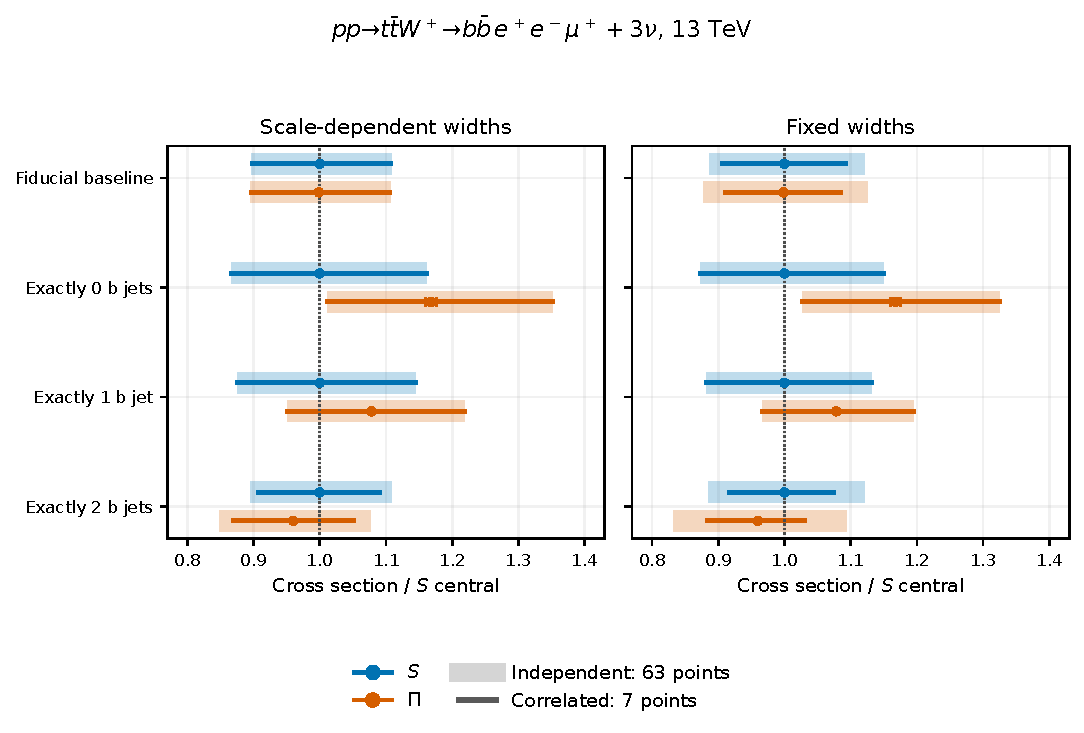
\includegraphics[width=\linewidth]{01_rates.pdf}
\caption{Baseline-selected total and exclusive tag rates. Each
horizontal unit is the $S$ mean central value in that selection and
width convention. Thick light intervals show I63 and thin solid
intervals C7. Markers carry propagated native MC errors. The plotting
reference does not assign an independent error to a ratio.}
\label{fig:rates}
\end{figure}

\clearpage
\begin{figure}[htbp]\centering
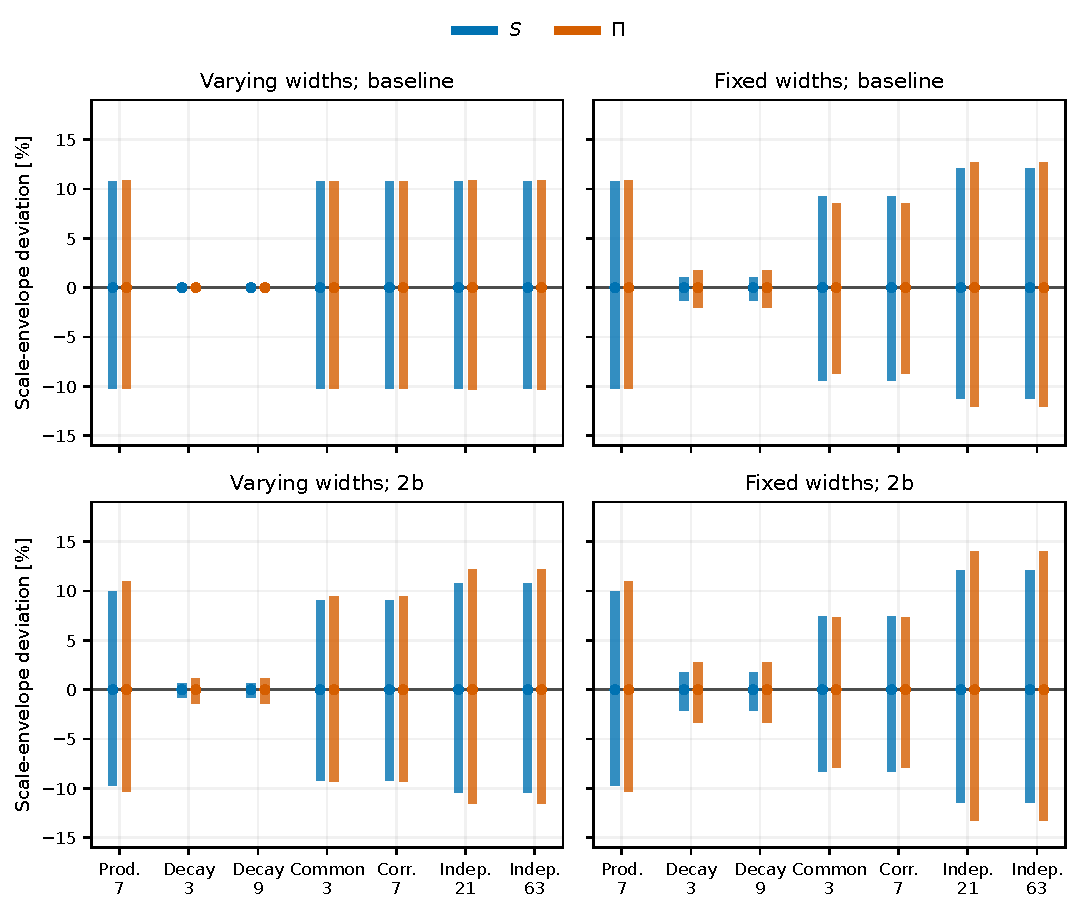
\includegraphics[width=\linewidth]{02_scale_prescriptions.pdf}
\caption{Alternative scale envelopes for the baseline total and
two-tag rate. Each interval is measured relative to its own central
prediction; markers sit at zero. Freezing widths strengthens the
opposing decay response and reduces the envelope when scales are tied.
The separate decay axes do not enlarge these particular integrated
extrema.}
\label{fig:scales}
\end{figure}

\clearpage
\begin{figure}[htbp]\centering
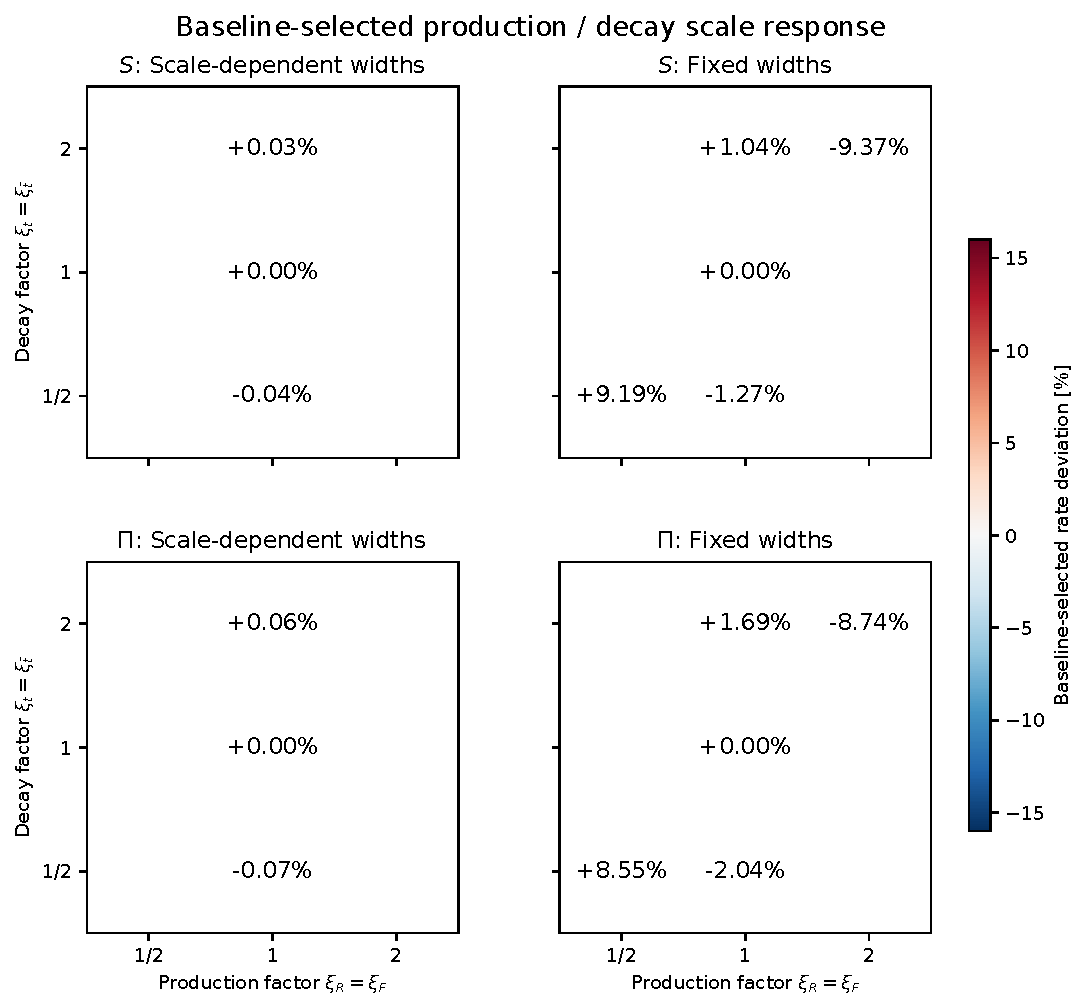
\includegraphics[width=.92\linewidth]{03_scale_response.pdf}
\caption{Baseline-selected production/decay response slices, with
$\xi_R=\xi_F$ and $\xi_t=\xi_{\bar t}$. Cells give deviations from
the corresponding central mean. Common3 follows the diagonal;
independent variations also reach off-diagonal cells. The response is
computed from the averaged scale weights and is not a covariance or
likelihood.}
\label{fig:response}
\end{figure}

\clearpage
\begin{figure}[htbp]\centering
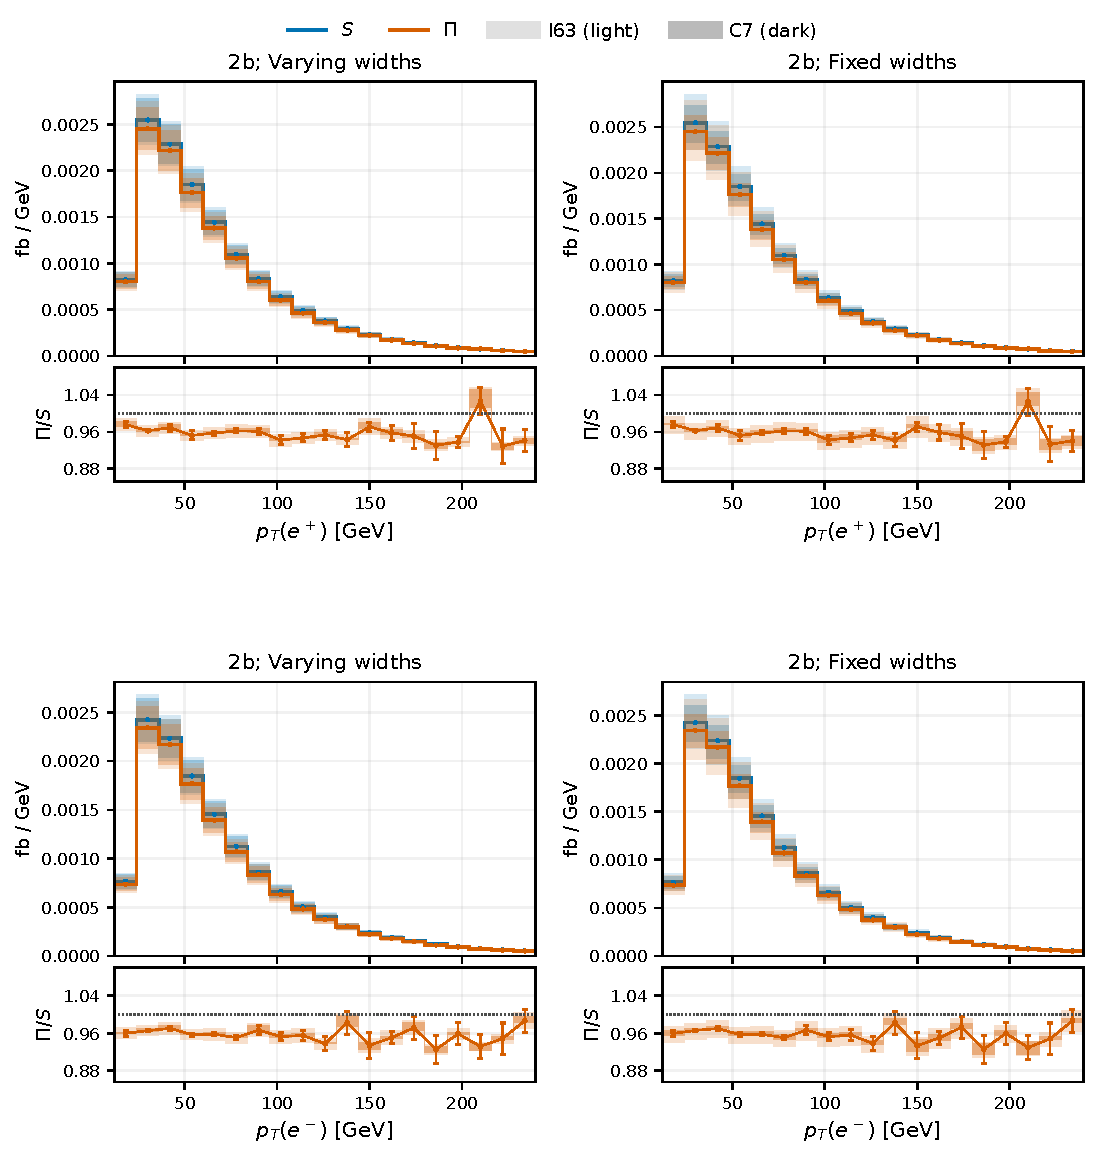
\includegraphics[width=\linewidth]{04_lepton_pt.pdf}
\caption{Two-tag electron and positron transverse momenta. Left:
scale-dependent widths; right: fixed widths. Absolute densities carry
propagated native MC bars, light I63 and darker C7 shading. Ratio
panels carry paired-replica jackknife MC bars and point-matched scale
envelopes. Native bins are retained, including bins straddling the
20 GeV lepton cut.}
\label{fig:leptons}
\end{figure}

\clearpage
\begin{figure}[htbp]\centering
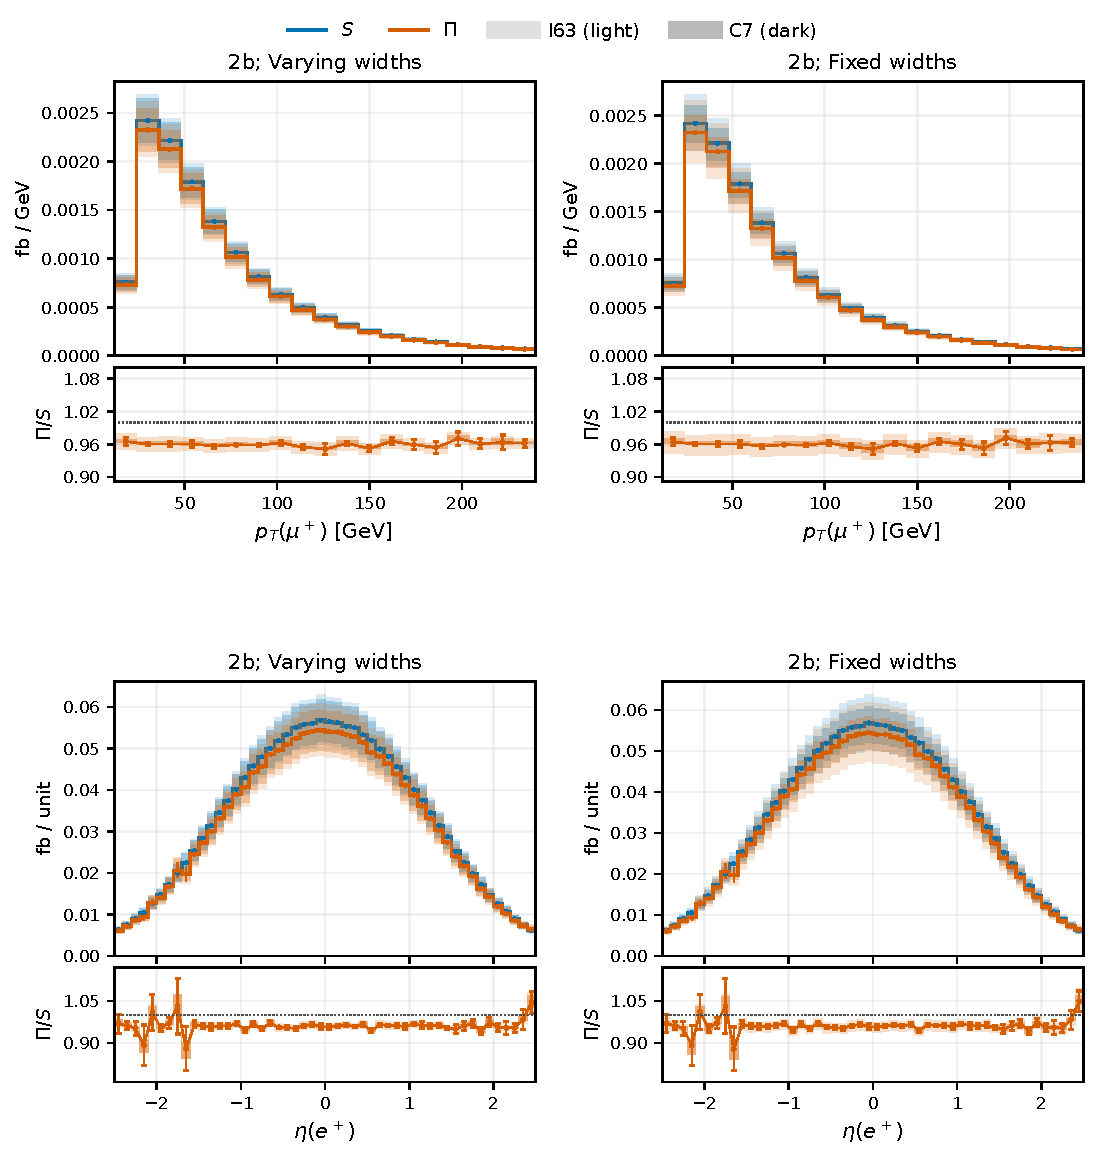
\includegraphics[width=\linewidth]{05_muon_eta.pdf}
\caption{Two-tag associated-muon transverse momentum and positron
pseudorapidity, with the conventions of Fig.~\ref{fig:leptons}.
The muon probes production and spin information; the top-decay positron
also responds directly to decay acceptance. Every charged lepton has
the same $\pt\geq20$ GeV and $|\eta|<2.5$ acceptance.}
\label{fig:muon}
\end{figure}

\clearpage
\begin{figure}[htbp]\centering
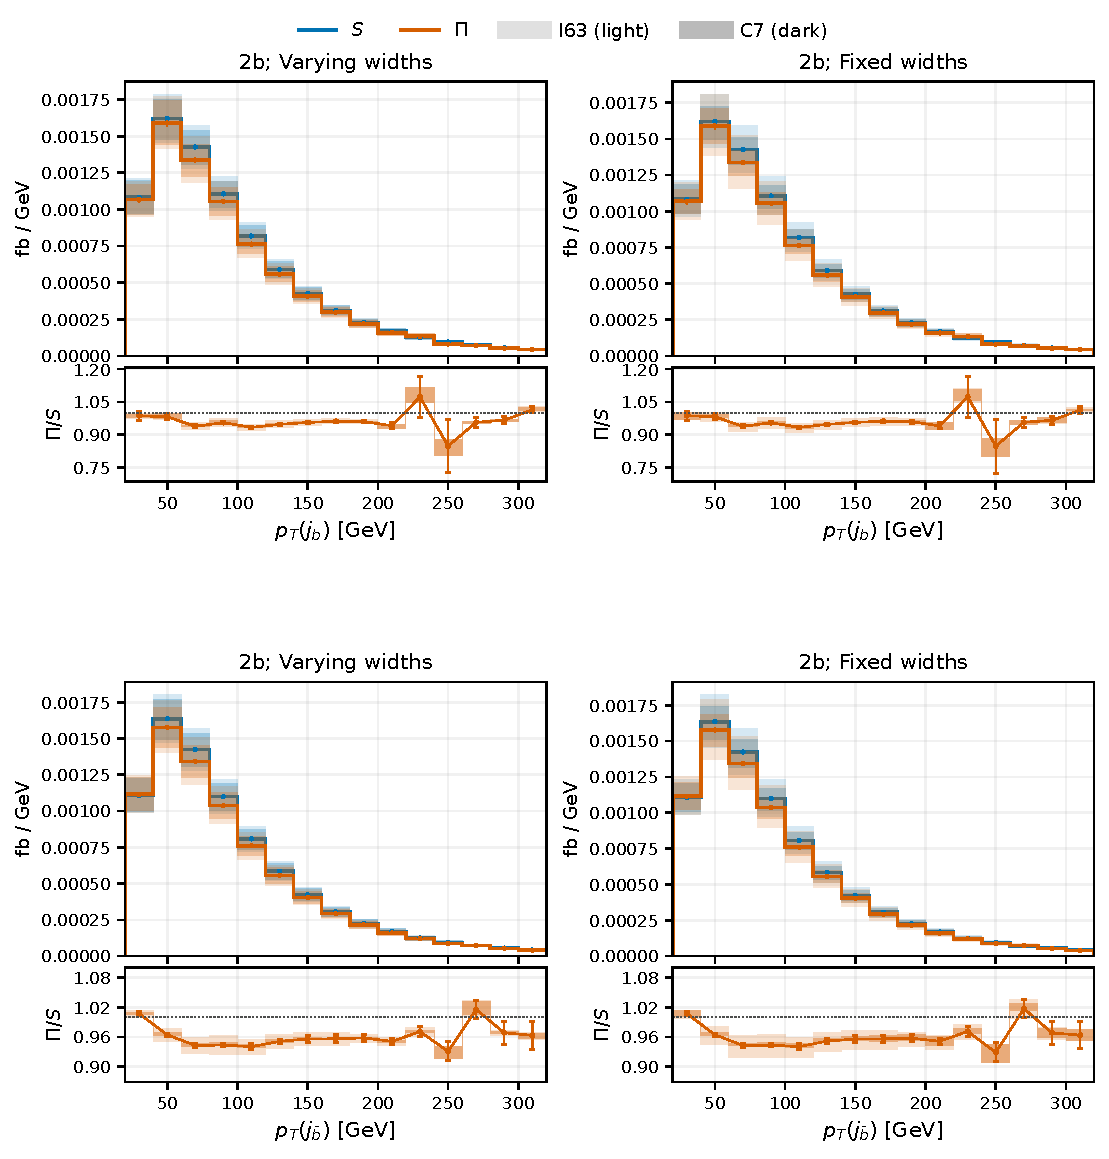
\includegraphics[width=\linewidth]{06_bottom_pt.pdf}
\caption{Separate accepted bottom- and antibottom-jet transverse
momenta in the two-tag category. Jets containing both bottom flavours
do not enter these distributions. Uniform lepton and jet acceptance
does not impose identical spectra in the charge-asymmetric $W^+$
process. The densities are not shape-normalized.}
\label{fig:bottom}
\end{figure}

\clearpage
\begin{figure}[htbp]\centering
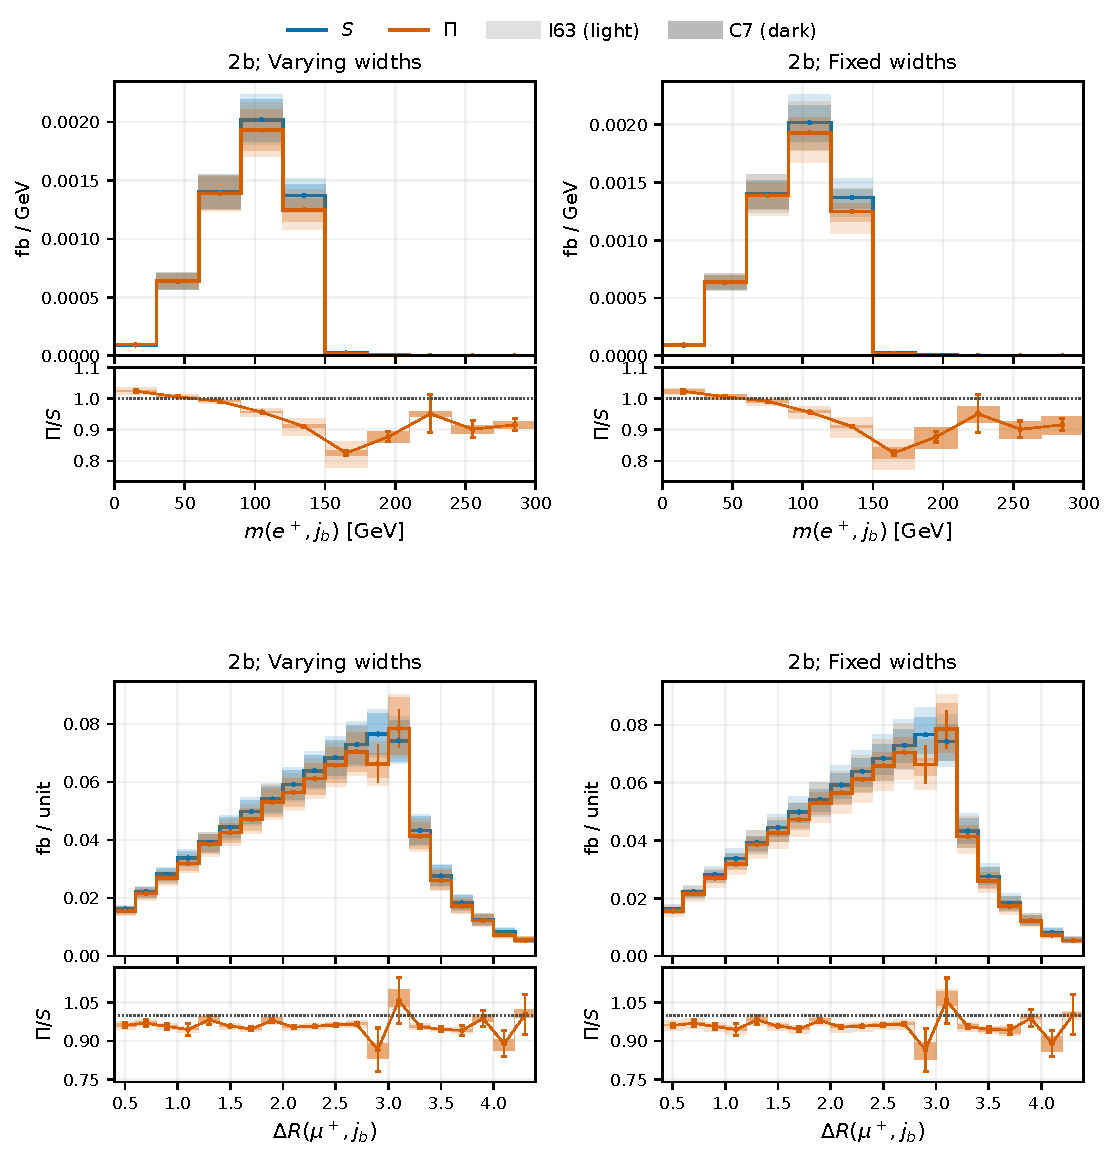
\includegraphics[width=\linewidth]{07_lepton_bottom.pdf}
\caption{Two-tag $m(e^+,j_b)$ and $\Delta R(\mu^+,j_b)$, with
absolute and ratio uncertainties as in Fig.~\ref{fig:leptons}.
The mass uses the top-decay positron and the jet containing its bottom
parton in this direct-lepton assignment. Jet radiation can populate
bins beyond the approximately 152.6 GeV Born endpoint. The angular
combination supplies a complementary directly visible correlation.}
\label{fig:lepb}
\end{figure}

\clearpage
\begin{figure}[htbp]\centering
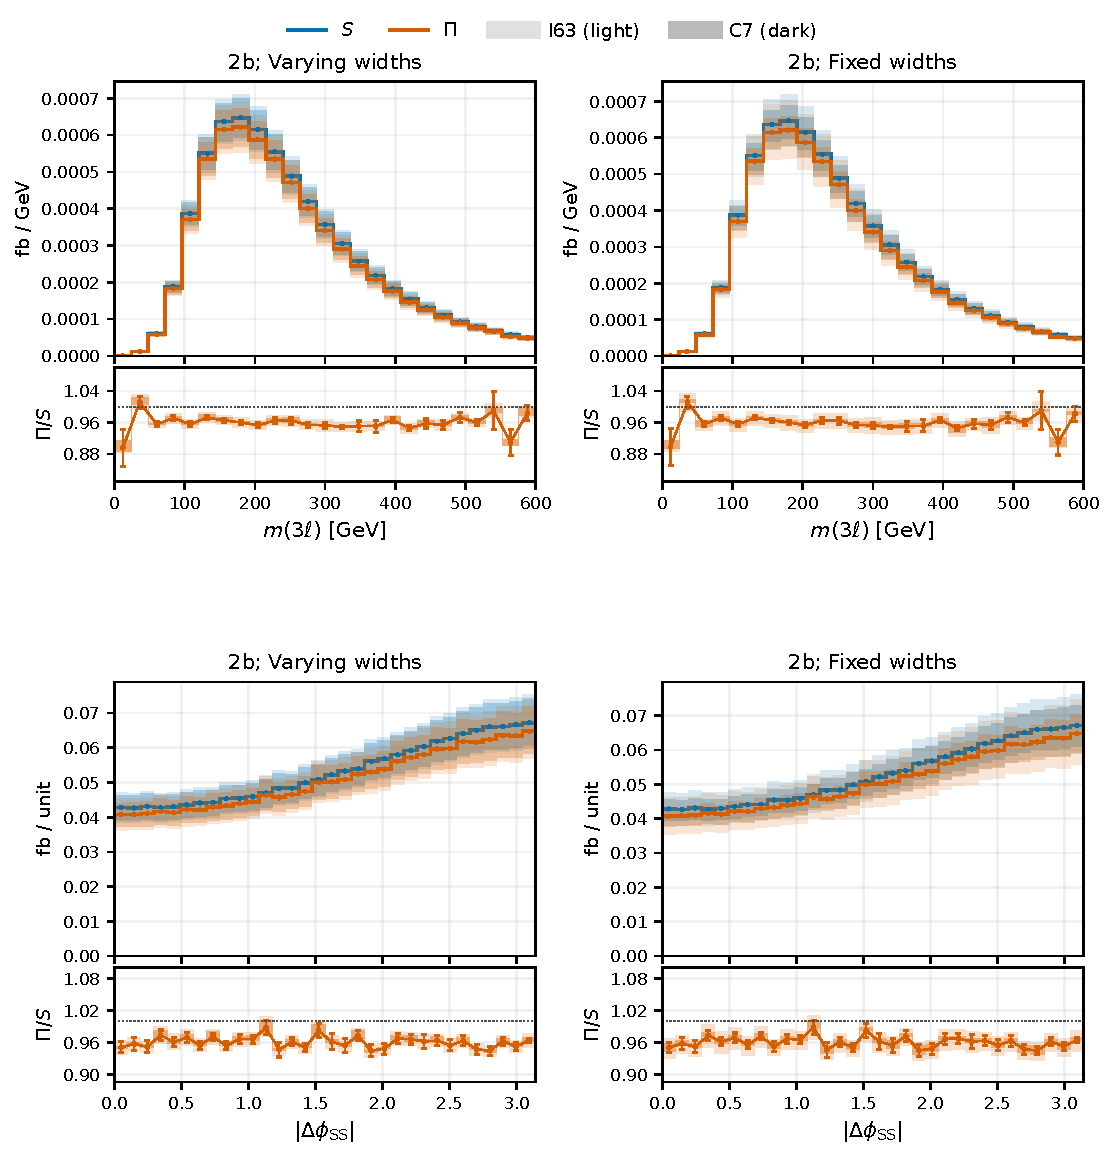
\includegraphics[width=\linewidth]{08_trilepton_angles.pdf}
\caption{Two-tag trilepton invariant mass and same-sign azimuthal
separation. Here the same-sign pair is $e^+\mu^+$. There is no Z-mass
veto. These combinations require no neutrino fit or reconstructed
parent assignment. Scale shading and paired statistical bars are
distinct uncertainty estimates.}
\label{fig:trilepton}
\end{figure}

\clearpage
\begin{figure}[htbp]\centering
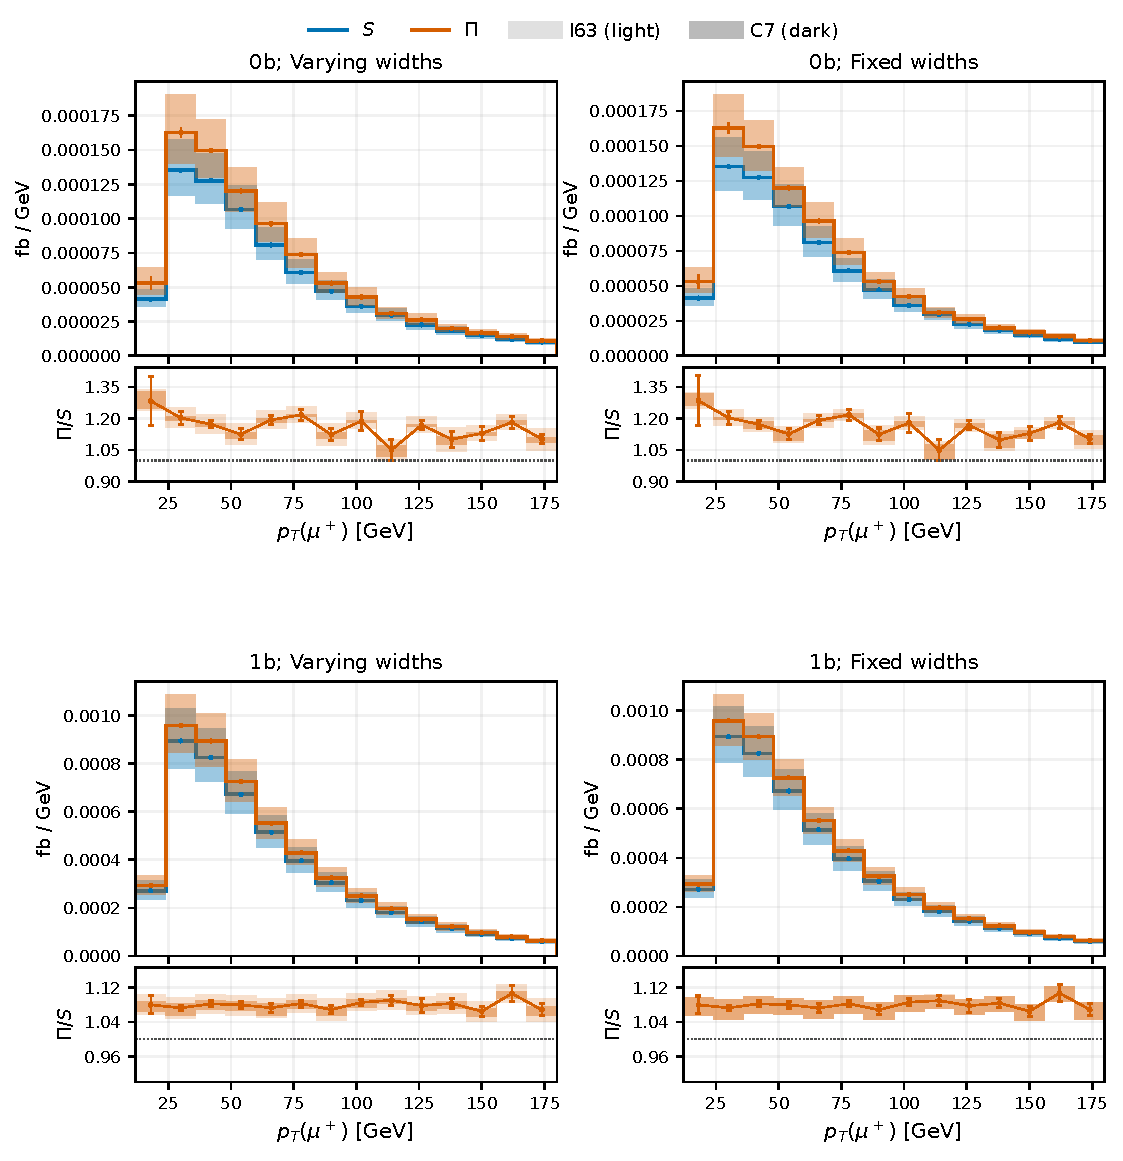
\includegraphics[width=\linewidth]{09_low_tag_categories.pdf}
\caption{Associated-muon transverse momentum in the exclusive
zero-tag and one-tag categories. Their multiplicative enhancements
are visible at substantially improved precision. Rare zero-tag bins
remain less precise; no smoothing or removal of populated native bins
is used. Ratio bars estimate MC precision from paired replicas and
must not be confused with the shaded scale envelopes.}
\label{fig:lowtags}
\end{figure}

\clearpage
\begin{figure}[htbp]\centering
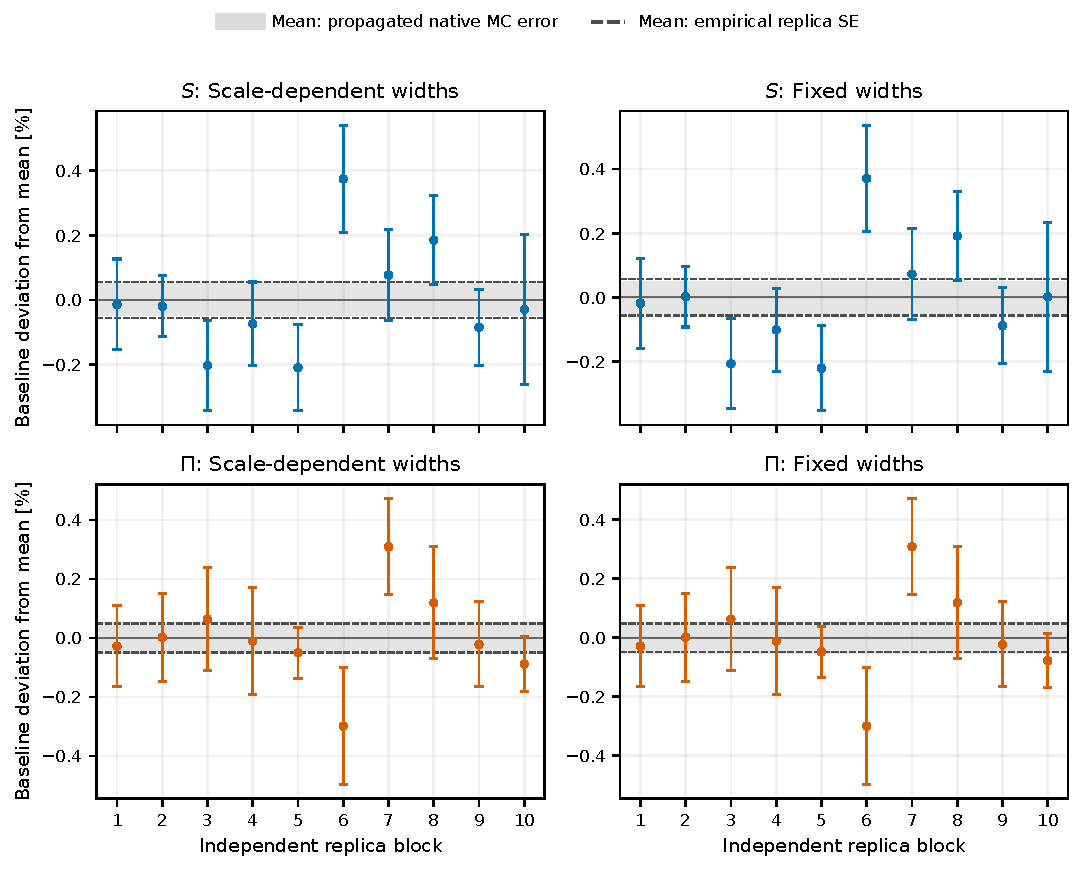
\includegraphics[width=\linewidth]{10_replica_precision.pdf}
\caption{Baseline rate in each repeated integration, relative to
its ten-replica mean. Bars show the native error of each integration.
The grey interval is the propagated native error on the mean and
dashed lines show the empirical standard error on the mean. Width
partners share most streams, so these panels are not four independent
ensembles for cross-prediction comparisons.}
\label{fig:replicas}
\end{figure}

\clearpage
\appendix
\section{Reproducibility and scope}
The report directory contains this LaTeX source and PDF, five generated
tables, ten PDF/PNG figures, archived cards for all forty integrations,
installed source snapshots, the numerical \code{results.json}, the
combined \code{collected.npz}, figure and report manifests, and the
full-catalogue precision CSV. The combined arrays retain the central
and native error of every replica in every bin, the empirical error
on each mean, and all 81 mean scale weights. Original run files are
read-only inputs. Their paths and hashes are recorded.

Collection verifies complete compatible histogram layouts and scale
coordinates, matched reference cards, fixed-width inputs, the central
scale weight, and tag-category closure. It also checks that different
replica blocks have no shared logged seed pairs. These are consistency
checks and a sampling audit, not a proof of convergence in every tail.
The combined sample retains native bins: no unsupported within-run
quadrature rebinning or artificial smoothing is used. The signed decay
labels print \code{d-6} before \code{d6}; the reduction explicitly
orders coordinates as production $\mu_R$, production $\mu_F$, top
$\mu_R$, antitop $\mu_R$.

From the repository root, reproduce the reduction and figures with
\begin{verbatim}
python ttw_study/scripts/collect_decay_scale_report.py \
  --campaign-root . --output ttw_study/reports/decay_scales_20261030
python ttw_study/scripts/render_decay_scale_report.py \
  --output ttw_study/reports/decay_scales_20261030
cd ttw_study/reports/decay_scales_20261030
make
\end{verbatim}
The source ZIP contains the document, generated table inputs, standalone
PDF figures and build instructions, sufficient to rebuild the report.
The larger numerical arrays and original HwU files are not required
merely to compile that ZIP. The report prose is specific to these
inputs and should be reviewed if the campaign is changed.

This sample does not include a direct-lepton-flavour sum, $W^-$,
PDF uncertainty, non-factorizable or finite-width corrections,
electroweak corrections, parton-shower matching or a complete NNLO
calculation. Existing full off-shell results provide comparison targets
under matched conditions; they have not been rerun with these cuts.
The earlier neutrino-fit observables remain retired. Statistical
fluctuations or endpoint sensitivity in the present visible observables
do not by themselves establish a new infrared-safety failure.

\begin{thebibliography}{9}
\bibitem{MG5} J. Alwall et al.,
\emph{The automated computation of tree-level and next-to-leading order
differential cross sections, and their matching to parton shower simulations},
JHEP 07 (2014) 079, \href{https://arxiv.org/abs/1405.0301}{arXiv:1405.0301}.
\bibitem{MadFKS} R. Frederix, S. Frixione, F. Maltoni and T. Stelzer,
\emph{Automation of next-to-leading order computations in QCD: the FKS subtraction},
JHEP 10 (2009) 003, \href{https://arxiv.org/abs/0908.4272}{arXiv:0908.4272}.
\bibitem{ttW2020} G. Bevilacqua, H.-Y. Bi, H. B. Hartanto, M. Kraus and M. Worek,
\emph{The simplest of them all: $t\bar tW^\pm$ at NLO accuracy in QCD},
JHEP 08 (2020) 043, \href{https://arxiv.org/abs/2005.09427}{arXiv:2005.09427}.
\bibitem{ttWmodel} G. Bevilacqua et al.,
\emph{Modeling uncertainties of $t\bar tW^\pm$ multilepton signatures},
Phys. Rev. D 105 (2022) 014018,
\href{https://arxiv.org/abs/2109.15181}{arXiv:2109.15181}.
\bibitem{ttWNNLO} L. Buonocore et al.,
\emph{Precise predictions for the associated production of a W boson
with a top-antitop quark pair at the LHC},
Phys. Rev. Lett. 131 (2023) 231901,
\href{https://arxiv.org/abs/2306.16311}{arXiv:2306.16311}.
\bibitem{ttWNNLO2026} M. Becchetti et al.,
\emph{NNLO QCD predictions for $t\bar tW$ production at hadron colliders},
\href{https://arxiv.org/abs/2606.09503}{arXiv:2606.09503}.
\end{thebibliography}
\end{document}
